\section{Resultados}
\label{sec:resultados}

En esta sección se presentan los resultados de PSO sobre la función F5 (Shifted and Rotated Rastrigin) del benchmark CEC 2017 en 10, 20 y 30 dimensiones. Cada configuración del coeficiente de inercia $w$ se ejecutó 30 veces con 50 partículas y 1000 iteraciones. La ejecución $k$ de cada configuración partió de la misma población inicial, de modo que las diferencias entre configuraciones se deben a la estrategia de $w$ y no a la inicialización. La métrica reportada es el error $f(x_{best}) - f^*$, donde $f^* = 500$ es el valor óptimo de F5. Ninguna ejecución alcanzó el óptimo global; el error más bajo registrado fue de 4.97, obtenido con $w$ lineal decreciente en $D=10$.

\subsection{Error final por configuración}

La Tabla~\ref{tab:pso_rastrigin} resume la media y la desviación estándar del error final. La mejor configuración de cada dimensión aparece en negritas. El símbolo entre paréntesis indica el resultado de la prueba de Wilcoxon pareada contra la mejor configuración, con corrección de Holm y $\alpha = 0.05$: (+) significa que la mejor configuración es significativamente superior y (=) que la diferencia no es significativa.

\begin{table}[H]
\centering
\caption{Error $f(x_{best})-f^*$ de PSO en F5 (Rastrigin) (media $\pm$ desviación estándar, 30 ejecuciones).}
\label{tab:pso_rastrigin}
\resizebox{\textwidth}{!}{%
\begin{tabular}{lccc}
\toprule
Configuración de $w$ & $D=10$ & $D=20$ & $D=30$ \\
\midrule
Constante $w=0.4$ & 29.442 $\pm$ 13.060 (+) & 72.037 $\pm$ 19.543 (+) & 185.764 $\pm$ 48.687 (+) \\
Constante $w=0.6$ & 25.764 $\pm$ 8.035 (+) & 64.029 $\pm$ 18.045 (+) & 139.393 $\pm$ 41.407 (+) \\
Constante $w=0.7298$ & 16.804 $\pm$ 5.990 (=) & 55.078 $\pm$ 20.177 (+) & 123.156 $\pm$ 33.203 (+) \\
Constante $w=0.9$ & 26.465 $\pm$ 6.849 (+) & 91.607 $\pm$ 16.288 (+) & 222.272 $\pm$ 21.899 (+) \\
Lineal $0.9\to0.4$ & \textbf{14.538 $\pm$ 5.690} & \textbf{37.764 $\pm$ 13.615} & \textbf{82.609 $\pm$ 29.148} \\
Fitness $1.1r/f(x)$ & 39.460 $\pm$ 12.969 (+) & 101.298 $\pm$ 23.609 (+) & 251.794 $\pm$ 40.230 (+) \\
Fitness $1.1r/\text{error}$ & 41.274 $\pm$ 12.024 (+) & 104.239 $\pm$ 22.745 (+) & 248.884 $\pm$ 38.504 (+) \\
\bottomrule
\end{tabular}%
}
\end{table}

El $w$ lineal decreciente obtuvo el menor error medio en las tres dimensiones: 14.54 en $D=10$, 37.76 en $D=20$ y 82.61 en $D=30$. La segunda posición correspondió siempre al $w$ constante de 0.7298. En $D=10$ la diferencia entre ambas no fue significativa ($p = 0.088$), pero en $D=20$ y $D=30$ sí lo fue, y la distancia entre ellas creció con la dimensión. En $D=10$ el error de $w=0.7298$ es 16\,\% mayor que el de la estrategia lineal, mientras que en $D=20$ y $D=30$ es 46\,\% y 49\,\% mayor, respectivamente.

El enfoque basado en fitness tuvo el peor desempeño en todas las dimensiones. Sus dos variantes, con $f(x)$ y con el error $f(x)-f^*$ en el denominador, dieron resultados casi idénticos (39.46 frente a 41.27 en $D=10$ y 251.79 frente a 248.88 en $D=30$). En $D=30$ su error medio triplica el de la estrategia lineal.

La Figura~\ref{fig:barras} muestra los mismos datos en forma gráfica. La desviación estándar aumenta con la dimensión en todas las configuraciones. En $D=30$ la más baja corresponde a $w=0.9$ (21.90), aunque su media (222.27) es de las más altas.

\begin{figure}[H]
\centering
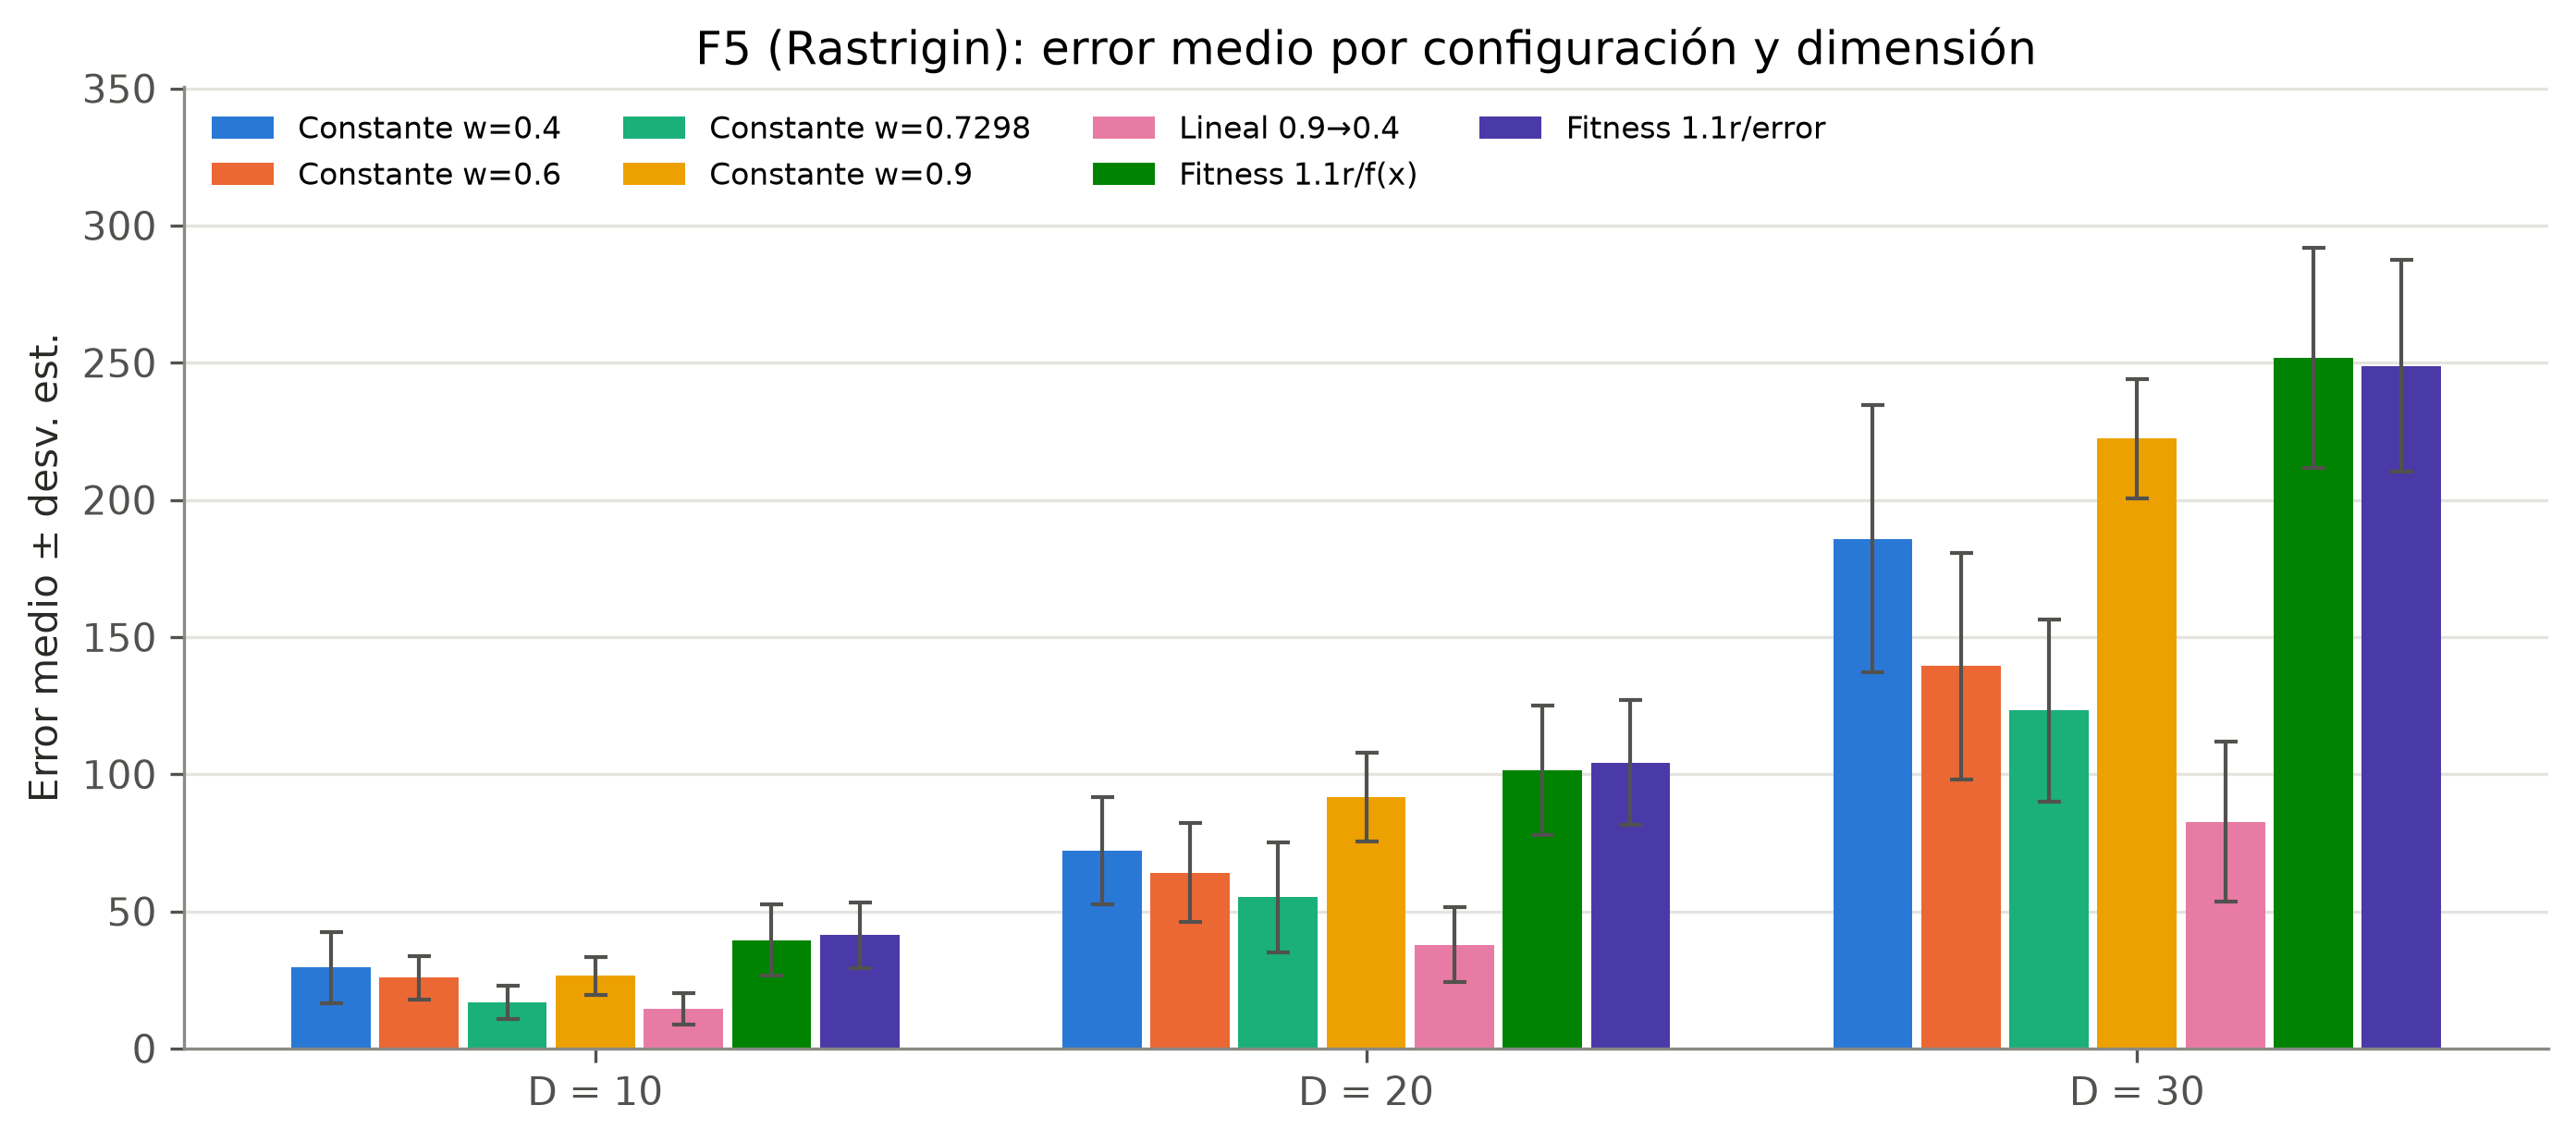
\includegraphics[width=\textwidth]{figuras/barras_media_desviacion.png}
\caption{Error medio $\pm$ desviación estándar de cada configuración de $w$ por dimensión.}
\label{fig:barras}
\end{figure}

\subsection{Distribución del error}

La Figura~\ref{fig:boxplots} muestra la distribución del error final de las 30 ejecuciones. En las tres dimensiones la caja de la estrategia lineal es la más baja, y en $D=20$ y $D=30$ su mediana (34.00 y 83.08) queda por debajo del primer cuartil de todas las demás configuraciones. En $D=30$ su tercer cuartil prácticamente coincide con el primer cuartil de $w=0.7298$.

Las dos variantes del enfoque basado en fitness tienen cajas similares entre sí y separadas del resto. En $D=10$ son además las de mayor dispersión, con errores entre 15 y 72. El $w$ constante de 0.4 también presenta una dispersión alta en las tres dimensiones y tiene la desviación estándar más grande de los valores constantes (13.06 en $D=10$ y 48.69 en $D=30$). Esto indica que su resultado depende mucho de la población inicial. Con $w=0.9$ ocurre lo contrario en $D=30$: la caja es estrecha pero está en un nivel de error alto, es decir, el algoritmo falla de manera consistente.

\begin{figure}[H]
\centering
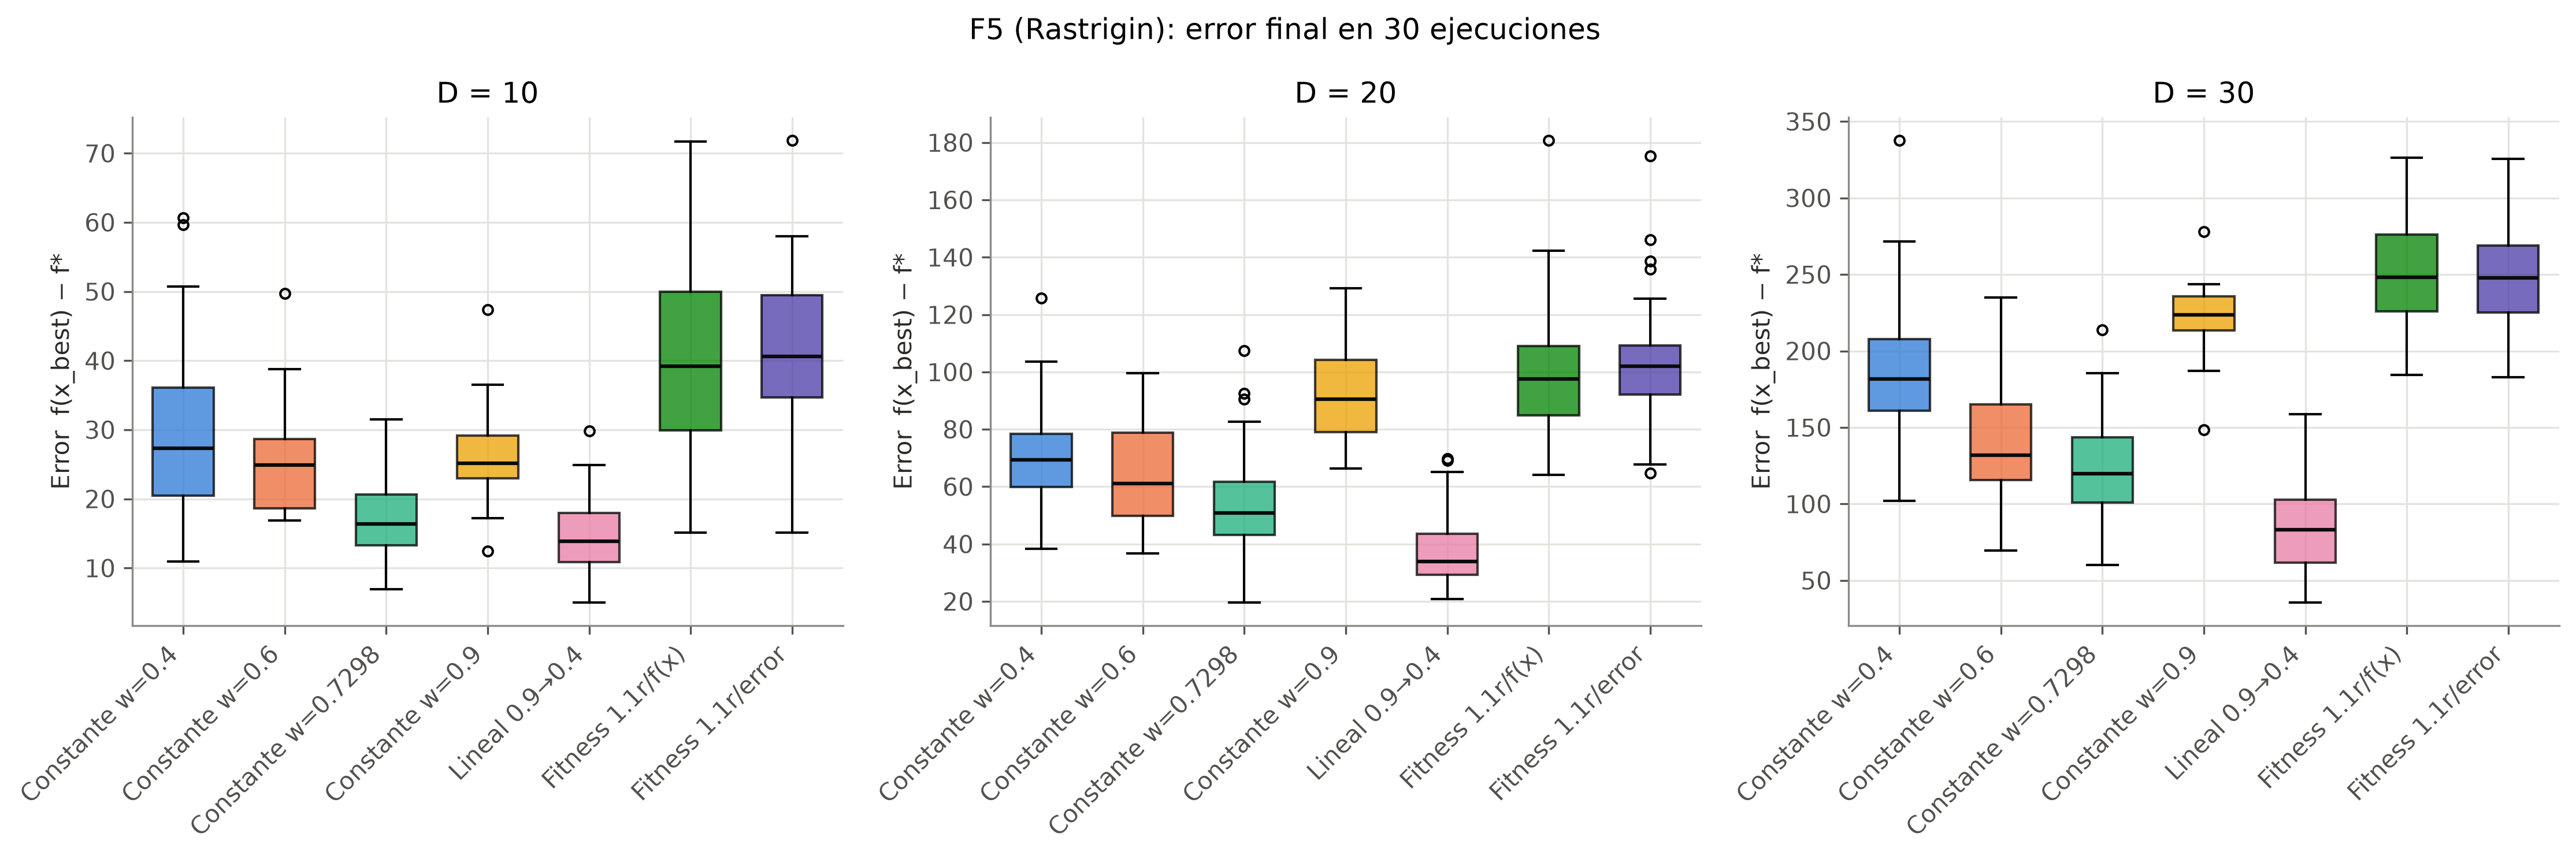
\includegraphics[width=\textwidth]{figuras/boxplots_error_final.png}
\caption{Distribución del error final en 30 ejecuciones para $D = 10$, 20 y 30.}
\label{fig:boxplots}
\end{figure}

\subsection{Sensibilidad al valor de \texorpdfstring{$w$}{w} y escalabilidad}

La gráfica izquierda de la Figura~\ref{fig:sensibilidad} muestra el error medio en función del valor de $w$ constante. En las tres dimensiones la relación tiene forma de U, con el mínimo en $w=0.7298$: valores menores provocan convergencia prematura y valores mayores impiden la convergencia. La forma se acentúa al aumentar la dimensión. En $D=10$ el error medio varía entre 16.80 y 29.44 según el valor de $w$, y en $D=30$ entre 123.16 y 222.27. Las líneas punteadas marcan el error de la estrategia lineal, que queda por debajo de todos los valores constantes probados en cada dimensión.

La gráfica derecha muestra cómo crece el error medio con la dimensión. Todas las configuraciones empeoran al pasar de 10 a 30 variables, y el crecimiento es más pronunciado entre $D=20$ y $D=30$ que entre $D=10$ y $D=20$. El orden de las configuraciones se mantiene casi igual en las tres dimensiones. La única excepción es $w=0.9$, que en $D=10$ tiene un error similar al de $w=0.6$ (26.46 frente a 25.76) y en $D=30$ es el peor de los valores constantes. La estrategia lineal pasa de 14.54 a 82.61, y es la configuración con menor error en todas las dimensiones.

\begin{figure}[H]
\centering
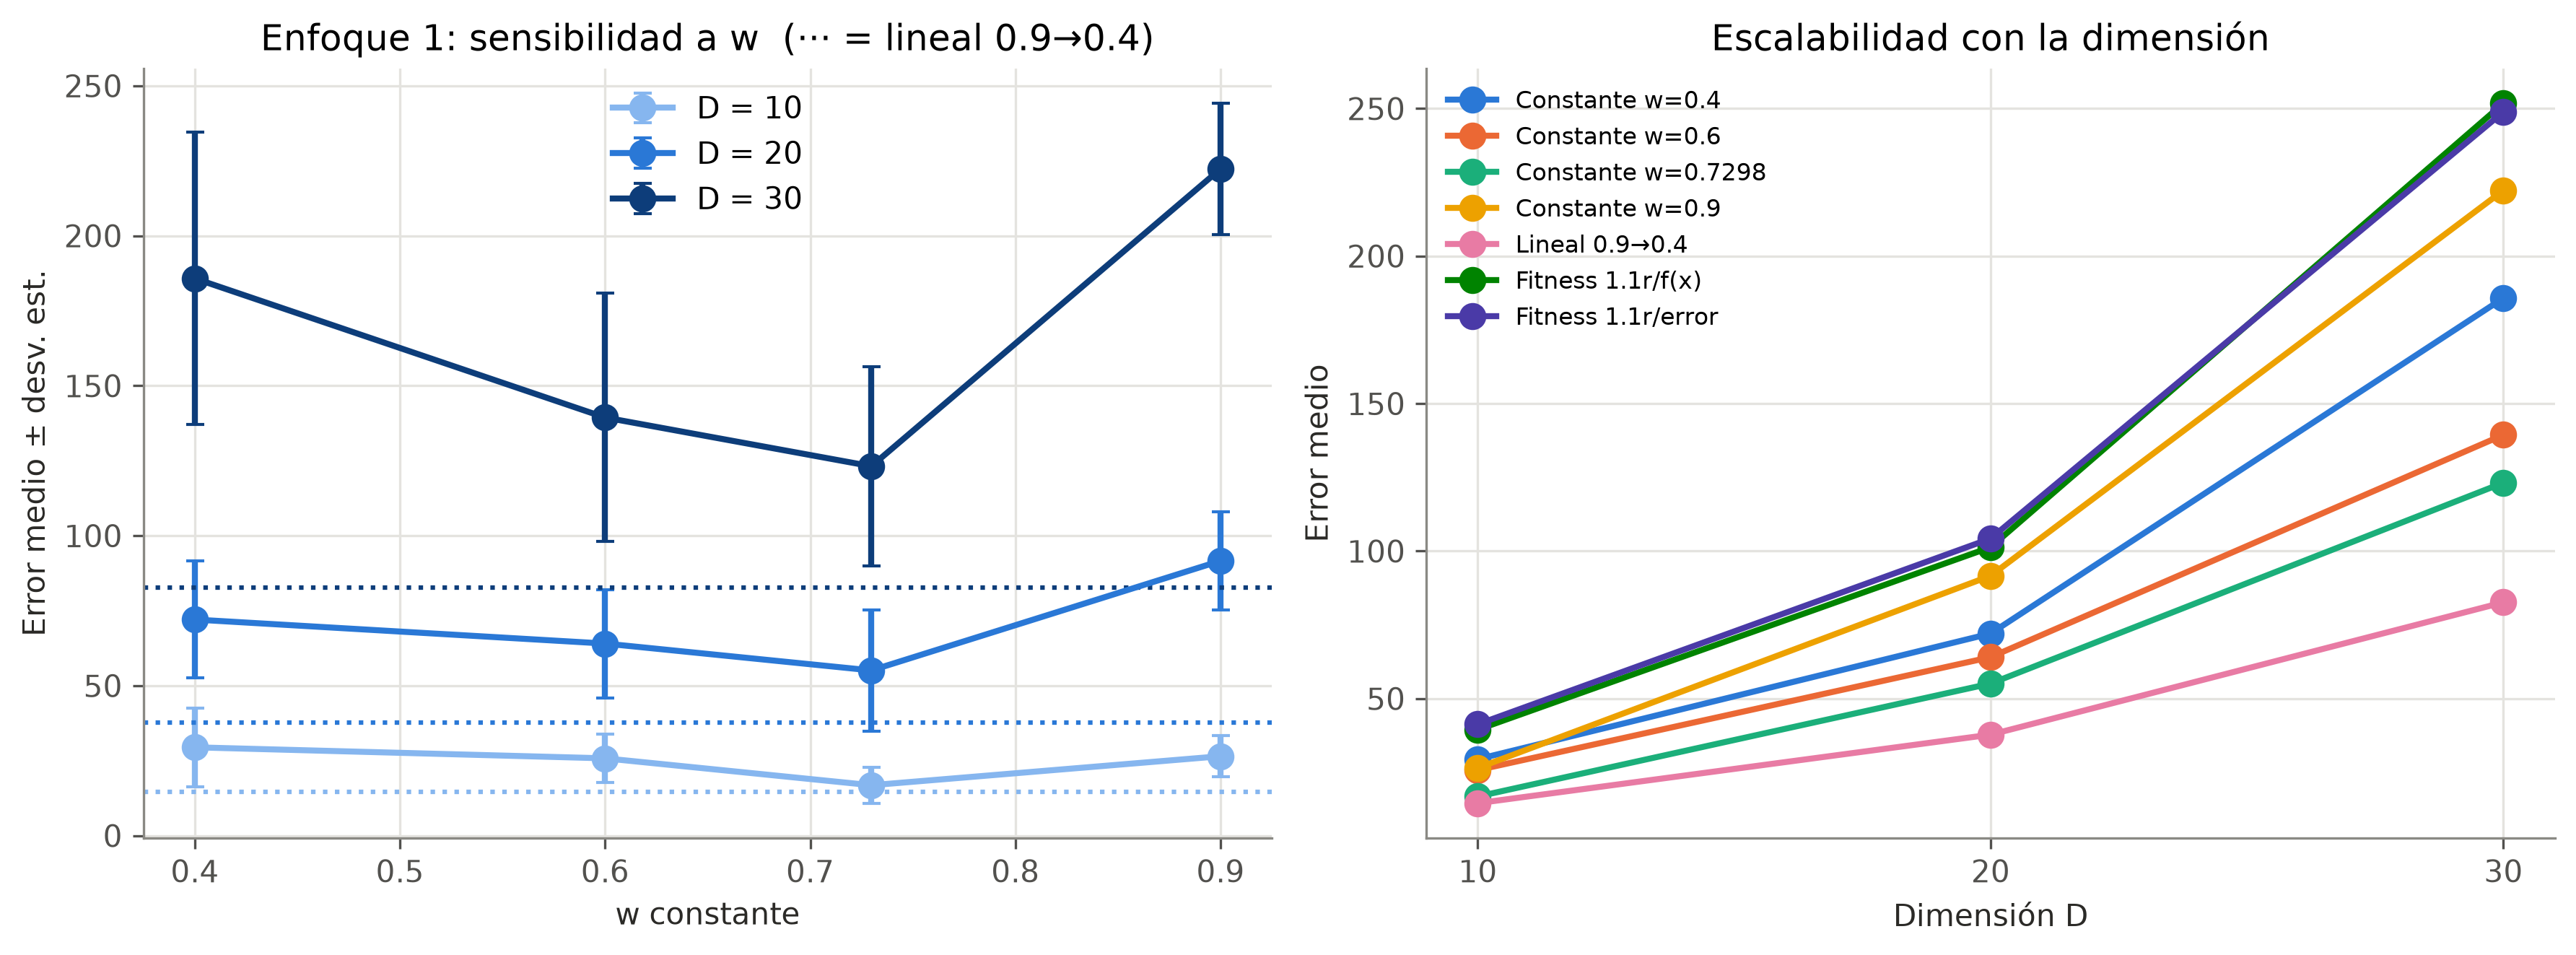
\includegraphics[width=\textwidth]{figuras/sensibilidad_y_escalabilidad.png}
\caption{Izquierda: error medio en función de $w$ constante (las líneas punteadas corresponden a la estrategia lineal $0.9\to0.4$). Derecha: error medio en función de la dimensión.}
\label{fig:sensibilidad}
\end{figure}
